% !TEX encoding = UTF-8 Unicode
% !TEX root =  ../Main.tex

\chapter{Realisierung}\label{cha:prototyp}
Die Webanwendung soll auf der Website des \gls{asta} erscheinen. Da die aktuelle Website au WordPress basiert, müssen das Antragsformular als auch das Bearbeitungsportal mit diesem System kompatibel sein. WordPress ist ein \gls{cms}, das primär der Bereitstellund und Verwaltung von Inhalten dient. Neben dem Aufbau statischer und dynamischer Websites ermöglicht es das Management und die Verwaltung von Daten sowei die Speicherung von Dokumenten, Fotos, Videos und wieteren Formaten. WordPress ist beliebt, weil es auch für Personen ohne technischen Hintergrund leicht zu bedienen ist, eine große Auswahl an kostenlos verfügbaren Themes und Plug-ins anbietet und sich flexibel an unterscheidliche Anforderungen anpassen lässt. \VglZitat{kumarWordPressMultiFunctionalContent2021}{158 f.}

Für den Betrieb ist serverseitig die Verwendung von PHP7.4 oder höher sowie einer relationalen Datenbank MySQL5.7 oder MariaDB 10.3 oder höhrer notwendig.\VglZitat{AdvancedAdministrationHandbook2023}{} In diesem System wird MySQL verwendet. WordPress benötigt eine Datenbank, deshalb ist es sinnvoll ein zusätzliches Tool zur Verwaltung dieser einzusetzen. In dieser Lösung wird Adminer verwendet. Nach dem Login können dort sämtliche Datensätze eingesehen und verwaltet werden, was das Erstellen, Bearbeiten, Löschen und Exportieren von Daten einschließt. 

Um die Anwendung später auf einem Server bereitstellen zu können, wird die Zielumgebung in der Entwicklung mit Docker simuliert. DAs ermöglicht eine reproduzierbare lokale Entwicklungsumgebung, die sich später auf den Server übertragen lässt. Die verwendeten Images für WordPress, die MySQL Datenbank sowie adminer stammen aus dem offiziellen Docker Hub Registry. Die Konfiguration erfolgt über die docker-compose, wobei die Umgebungsvariablen zur Sicherheit in einer .env-Datei gespeichert werden (siehe Listing~\ref{lst:dockercompose} ). \\ 

\begin{lstlisting}[language=yaml,caption={docker-compose.yml Beispiel},label={lst:dockercompose}]
services:
  WordPress:
    image: WordPress:php8.1-apache
    container_name: WordPress
    ports:
      - "8080:80"
    environment:
      WordPress_DB_HOST: ${WordPress_DB_HOST}
      WordPress_DB_NAME: ${WordPress_DB_NAME}
      WordPress_DB_USER: ${WordPress_DB_USER}
      WordPress_DB_PASSWORD: ${WordPress_DB_PASSWORD}
      WordPress_DEBUG: ${WordPress_DEBUG}
      WordPress_TABLE_PREFIX: ${WordPress_TABLE_PREFIX}
    volumes:
      - ./wp-content:/var/www/html/wp-content
    depends_on:
      - db

  db:
    image: mysql:8
    container_name: mysql
    environment:
      MYSQL_ROOT_PASSWORD: ${MYSQL_ROOT_PASSWORD}
      MYSQL_DATABASE: ${MYSQL_DATABASE}
      MYSQL_USER: ${MYSQL_USER}
      MYSQL_PASSWORD: ${MYSQL_PASSWORD}
    ports:
      - "3307:3306"
    volumes:
      - db_data:/var/lib/mysql

  adminer:
    image: adminer
    container_name: adminer
    restart: always
    ports:
      - 8081:8080

volumes:
  db_data:
\end{lstlisting}

WordPress hat sowohl ein Backend als auch Frontend. Dass Frontend ist die Website, die die Nutzer:innen zu Gesicht bekommen. In diesem Fall die Studierenden. Das Backende von WordPress ist der Administrationsbereich der Seite(n). Hier können verschiedene Nutzerrollen angelegt werden, die Optionen für die Website konfiguriert werden und Erweiterungen wie Themes und Plug-ins installiert werden. Vor dem Zugriff auf das Backend muss man sich über eine Anmeldemaske anmelden. Je nach Benutzerrolle kann festgelegt werden, welche Bereiche des Administrationsbereichs angezeigt werden. \VglZitat{steyerWordPressEinfuehrungContent2016}{93 ff.}

Wie bereits angesprochen ist es möglich Themes und Plug-ins zusätzlich zu instalieren. Themes dienen der Designanpassung einer Seite. Durch die Veränderung des Themes kann es sein, dass Seiten vollkommen anders aussehen, andere Features bereitstellen und anderre Inhalte anzeigen. Das liegt daran, dass Wordpress jegliche Textinhalte einer Seite (Beiträge, Seiten, Kommentare) und Medien (Tondateien, Bilder, Videos) in Verzeichnissen ablegt, die von der Struktur einer Seite und deren Design abgetrennt sind. Das Design kann also individuell angepasst werden ohne den Inhalt zu verändern. \VglZitat{steyerWordPressEinfuehrungContent2016}{169}

Ein Plug-in ist eine Erweiterung der WordPress Seite, die im Hintergrund laufen und nicht zwingend zu sehen sein müssen. Ein solches Plug-in kann beispielsweise die Anzahl der Besucher einer Seite zählen, es kann die Datensicherunng vornehmen, es kann vor Spam schützen oder Suchmaschinenoptimierung vornehmen. Ein Plug-in kann aber auch im Frontend zu sehen sein und sogar wie eine normale Seite in WordPress integriert werden.  \VglZitat{steyerWordPressEinfuehrungContent2016}{191 ff.} Plug-ins erweitern die Funktionalitäten von WordPress. Sie werden mit der Programmiersprache PHP entwockelt und können weitere Ressourcen wie CSS oder JavaSkript beinhalten. Das macht die Entwicklung besonders flexibel. \VglZitat{WhatPluginPlugin2014}{}

Nach der Installation und Ausführung des des Wordpress Images über Docker ergibt sich die in Abbildung~\ref{fig:ordnerstruktur_wp} dargestellte Ordnerstruktur. Es ist zu erkennen, dass Themes sowie Plug-ins durch eigenen Code angepasst und neu hinzugefügt werden können.

\begin{figure}[htbp]
  \centering
  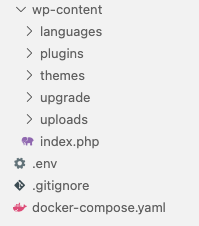
\includegraphics[width=0.3\textwidth]{Bilder/Ordnerstruktur_wp.png}
  \caption{Ordnerstruktur von WordPress nach Installation}\label{fig:ordnerstruktur_wp}
\end{figure}

- Antragsformular sowie Bearbeitungsportal sind mit einem solchen Plug-in realisiert
- aufbau der Strukturen: 
    - ein Plugin, welches die Datenbanktabellen so aufbaut, wie es modelliert wurde
    - ein Plugin für das Formular auf der AStA Website
    - Ein Plugin für das Bearbeitungsportal. Das soll im Adminbereich sein und mithilfe von Rollen entschieden werden, wer diese Seite dann sieht. 
    - es ergibt sich die folgende Ordnerstruktur: 
    \begin{figure}[htbp]
  \centering
  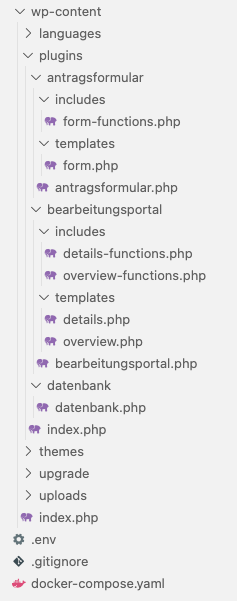
\includegraphics[width=0.3\textwidth]{Bilder/Ordnerstruktur_Projekt.png}
  \caption{Ordnerstruktur des Projektes mit den drei Plugins}\label{fig:ordnerstruktur_projekt}
\end{figure}

- es gibt hier also quasi ein Plugin für das Wordpress frontend (also die Seite die Studierende sehen) und ein Plugin für das Wordpress Backend also den Adminbereichn. Sowie eins für die Datenbank-Layer.
- Die ersten beiden Plugins sind aufgeteilt in die Hauptdatei, welche den Plugin Header beinhaltet und wenn notwendig hooks. Hier werden dann auch die notwendigen Funktionen aufgerufen. Die Business Logic (also aufgerufene Funktionen) weöche im Ordner includes gespeichert werden. 
- Das Datenbank Plugin hat nur die Hauptdatei, da hier keine Funktionen aufgerufen werden. 
- Neben den Funktionalitäten, also dem Backend haben das Plugin Antragsformular sowie das Plugin Antragsverwaltung jeweils einen templates ordner. Hier werden die HTMl-Vorlagen gespeichert, welche bestimmen wie das Plugin später angezeigt wird. Weil es in dem Bearbeitungsportal eine Überishctsseite und eine Antragsdetailansicht geben soll, gibt es zu jeder seite auch eine Businees Logik und ein HTML-Template. 


- Verwendung von Hooks. 
    -> basic hoks activation, deactivation und uninstall -> verweis auf wp seite zu plugins? \VglZitat{PluginBasicsPlugin2014}{}
    -> activation verwende ich beispielsweise in dem Bearbeitungsportal eine neue Art User namens "Sozialbüro" festzulegen,. nur die und admin können dann die anträge sehen und der administrator.  festzulegen, dass nur 
    -> hier eventuell screenshot
    -> das Datenbank plugin halt als activation hook die funktion, die die tabellen erstellt
    -> Deaktivate hooks sind hier nicht notwendig, auch uninstall nicht, da die Plugins auf der einen Seite zu simpel sind, auf der anderen Seite sollen keine Daten gelöscht werden. 

- Plugin header 
    -> das Plug-in wird mit PHP geschreiben. JEdes Datei brauct einen Header. Minimum ist heir der Plugin Name, welcher dann in dem Adminbereich von Wordpress angezegit wird. 
    -> es gibt noch ganz viele weitere Optionen, informationen über den Header mitzugeben. Ich habe mich jetzt aber nur für eine kurze Beschreibung, Autor und Versionentschieden


% -------------------------------DATENBANK--------------------------------
\section{Datenbank}\label{sec:Datenbank}
Das DatenbnK PLUGIN IST von den dreien das einfachste, denn es besteht nur aus einer einzigen PHP Datei. Es hat nur einen hook und zwar den zur Aktivierung des Plugins. Das liegt daran, dass bei der Deaktivierung oder Löschung keine DAten aus der Datenbank entfernt werden sollen. Die aufgerufene Funktion erstellt Datenbanktabellen nach dem entwickelten Datenbankschema. (hier Beispielhaft den Code für student). Es gibt eine sicherheitsfunktion, die darauf achtet, dass Tabellen nicht doppelt erstellt werden, wenn das Plugin deinstalliert und erneut installiert wird. Außerdem werden die Daten für die Antragsgründe, den Status und der Default Mitarbeiter "Leer" (als Person für die Historie wenn der Antrag neu eingereicht wird) direkt eingetragrn. 
Nach der Installation des Plugins sind die Tabellen über den DB Manager Adminer einsehbar. Hier können auch neue Daten hinugefügt oder gelöscht werden. -> Screenshot von Adminer?


% -------------------------------ANTRAGSFORMULAR--------------------------------
\section{Antragsformular}\label{sec:Antragsformular}
Das Antragsformular Plug-in ist im Gegensatz zur Datenbank etwas komplexer. In der Hauptdatei wird beschreiben, welches HTML-Formular angezeigt werden soll und was passiert, wenn ein Formular abgeschcikt wurde. Außerdem wird hier festgelegt, unter welchem Shortcode dieses Plugin auf einer Wordpress Seite aufgerufen werden kann. Dieser Shortcode hat also die Funtkionalität auf dem Frontend ein HTML Dokument auszugeben. 

Die aufgerufene HTML Datei ist relativ simpel gehalten. hier gibt es jetzt nicht so viel zu erklären. Das sieht halt ähnlich aus wie das Mockup, was ich gemacht hatte. Ein Bild davon ist dann im Anhang zu sehen. Die HTML Seite wird nicht direkt als HTML gspeichert sondern trotzdem in eine PHPDAtei. Deshalb ist es hier auch möglich gewesen ein dynamisches Element und zwar die Erfolgsnachricht bei Absenden eines Antrags anzuzeigen. Es gibt noch ein JS Element, das dafür sorgt, dass wenn das Häkchen "abweichender KOntoinhaber angeklcikt wird" ein Feld erscheint, in dem man eine schriftliche Bestätigung hochladen muss. 

Die letzte DAtei des Plugins ist dann die Business Logik. Hier befinden sich zum großteil Funktionen zur Validierung des Inhalts des abgeschcikten Formulars. Bei fFehlerm wird eine Benachrichtugng ausggeben. Es werden die Hochgeladenen Dokumente überprüft, der Inpt des Formulars wird überprüft, Daten werden vorbereitet und sanatized (siehe Kapitel xy), es wird überprüft ob der/die antragsstellende student:in schon existieert wenn nciht wird eine neue PErson angeleft, dann werden die Daten gespeichert, der Antragsstatus auf "Neu" gesetzt, die Dokumente hochgeladen und eine erfolgsnachricht geschcikt. alles auch mit Absicherungen sodass keine Fehler entstheen. 

% -------------------------------BEARBEITUNGSPORTAL--------------------------------
\section{Bearbeitungsprotal}\label{sec:Bearbeitungsprotal}


% -------------------------------_SECURITY--------------------------------
\section{Security}\label{sec:security}


???? was ist dieses :
// Prevent direct access
if (!defined('ABSPATH')) {
    exit; // Exit if accessed directly
}


    von WordPress selbst: 
        "When developing, it is important to consider security as you add functionality. Use the following principles as you progress through your development efforts: 
        • Don't trust any data. Don't trust user input, third-party APls, or data in your database without verification. Protection of your WordPress themes begins with ensuring the data entering and leaving your theme is as intended. Always make sure to validate and sanitize user input before using it, and to escape on output. 
        • Rely on the WordPress API. Many core WordPress functions provide the build in the functionality of validating and sanitizing data. Rely on the WordPress provided functions when possible. 
        • Keep your code up to date. As technology evolves, so does the potential for new security holes in your plugin or theme. Stay vigilant by maintaining your code and updating as required.
        
        Guiding principles 
        1. Never trust user input. 
        2. Escape as late as possible. 
        3. Escape everything from untrusted sources (e.g., databases and users), third-parties (e.g., Twitter), etc. 
        4. Never assume anything. 
        5. Sanitation is okay, but validation/rejection is better."

    - Wordpress gibt einige Security best Practices vor. 
    - Data sanatizing, bevor Daten gespeichert werden, wir überprüft, denn Daten können auch ungewollt falsch sein. Sanatizing ist dabei Proess von securing/cleaning/filtering input data
    - einen schritt weiter wäre data validating. Es geht hier also darum zu schauen, ob Daten einem bestimmten gewollten Muster folgen. Beispielsweise muss in dem Antrag IBAN, Matrikelnummer und Studimail angegeben werden. Alle diese Daten haben ein bestimmtes Ausssehen, so ist die IBAN nach einer DIN Richtlinie definiert, die Matrikelnummer besteht immer nur aus 11 Ziffern und die Studimail hat als ending @stud.hwr-berlin.de. es gehören auch so einfach sachen dazu wie zu checkem, dass alle Felder ausgefüllt wurden. 
    - Das überprüfen der Daten ist besonders in dem Plugin Antragsformular wichtig, denn hier geben Personen von außen (studierende) ihre Daten an, welche dann in die DB geschrieben werden. es wurden hier mehrere Prüffunktionen implementiert: 
    1. Überprüfung der Antragsgrößer (cap bei 5mb)
    2. Überprüfen der eingegebenen Daten
        -> wurden alle Felder ausgefüllt, wurden die Häkchen bei AGB und DAtenschutzbestimmungen gesetzt, ist die IBAn korrekt (überprüfung nach DIN norm), ist die BIC korrekt (korrekte verwendung von ZEichen, hat die MAtrikelnummer die richtige Länge, Wurden Dokumente hochgeladen.
    3. alle eingegebenen Daten sanitized und so eben überprüft.
    4. Es wird pberprüft, ob eine Person schon einen Antrag für das Semester gestellt hat (anhand von Matrikelnummer und Semester)

    - Verwendung von Nonces: Nonce steht für Number used once" und meint ein Zahl die durch Ihre einzigartigkeit URLS und Forms vor misuse, malicious und anderen schützt. Wordpress hingegen bestehen aus einem hash und werden für bestimmte ntuzer in einem bestimmten KOntext generiert. Das hilft dabei, vor einem Cross-Site Request Forgery (CSRF) zu schützen. \VglZitat{NoncesCommonAPIs2022}{}
    in diesem Projekt werden sie beispielsweise verwendetm wenn Nutzer einen Antrag über das Antragsformular stellen, Das führt dazu, dass keine Anträge über eine fremde Seite oder ein manupiliertest Sjrupt gestellt werden klnnen, welches auromatisch das formular ausfüllt und abschickt. Hier ist es also primär Schutz vor Spam. Nonces werden hier auch in der Antragsbearbeitung eingesetzt. DAs verhindert, dass unberechtigt Statusänderungen vorgenommen werden. 
    -> Code Beispiel

    - User roles. WordpRess unterstützt die verwendung eines Rollenkonzeptes. Es gibt bereits bereitgestellte Rollen wie Mitarbeiter, Admin etc. es gibt aber auch die möglichkeit eigene Rollen zu erstellen und diesen dann betimmte Rechte zu geben. So wurde in dem Bearbeitungsportal Plugin beispielsweise die Rolle Sozialbüro erstellt, welche neben dem Admin als einzige die Antragsseite im Administrationsbereich von WordPress sehen kann. Wurde diese Rolle angelegt, muss Sie noch manuell in das DB System aufgenommen werden und aufgrund des übereinstimmenden Namens können auch direkt Anträge bearbeitet werden. Das führt dazu, dass zum einen keine Unberechtigten die Daten einsehen können und auch die Anträge nicht ausversehen von anderen Mitarbeitenden berbeitet werden können. Es wird zusätzlich durch Funktionen im Code überprüft, ob eine PEson berechtigt ist, den Status zu verändern oder sich die Seite anzuschauen. 
    -> hier Code Beispiel hin 


    - Schutz gegen SQL injection: um SQL injection zu vermeiten gibt es eigene WorpPress Funktionen, mit denen eine SQL Abfrage sicher ausgeführt werden kann. Die zwei im Projekt verwendeten sind prepare() und insert(). Prepare() verwendet Platzhalter wie %d oder %s anstatt Varuablen direkt in den SQL String einzusetzen. WordPress ersetzt diese Platzhalter dann automatisch in die übergebenen Werte. 
    -> insert () hingegen sorgt dafür, dass kein SQl string übergeben wird sondern ein Array, der Spalten bestimte Werte zuordnet. Die Daten werden dann gecleaned und korrekt an die Datenbank übergeben. 

    - Cross Site Scripting verhinder: Hier wird code in die Website eingeschleust, was die Interaktion des Users mit der Website verändern kann. Sogenanntes Escaping trägt dazu bei, dass Daten vor der Ausgabe in HTML in reinen Text umgewandlet werden. Auführbarer Code wird vorher entfertn. Der/die Nutzer:in kann also nicht merh mit dem Code interagieren. Worpress bieter dafür je nach Typ unterschiedliche Funktionen. -> Hier Code Beispiel. Dort ist zu sehen, dass Werte, die aus der Datenbank angezeigt werden, mithilfe dieser Funktion als reiner ext angezeigt werden. 


